
\chapter{Projet \texttt{ILC}}

\section{Présentation du Projet ILC}

Le projet ILC (International Linear Collider) est un collisionneur linéaire, électron-positron, de 31 km conçu pour atteindre une énergie de centre de masse de 500 \GeV \cite{cern:ilc}. \\

\begin{figure}[h!]
	\center
	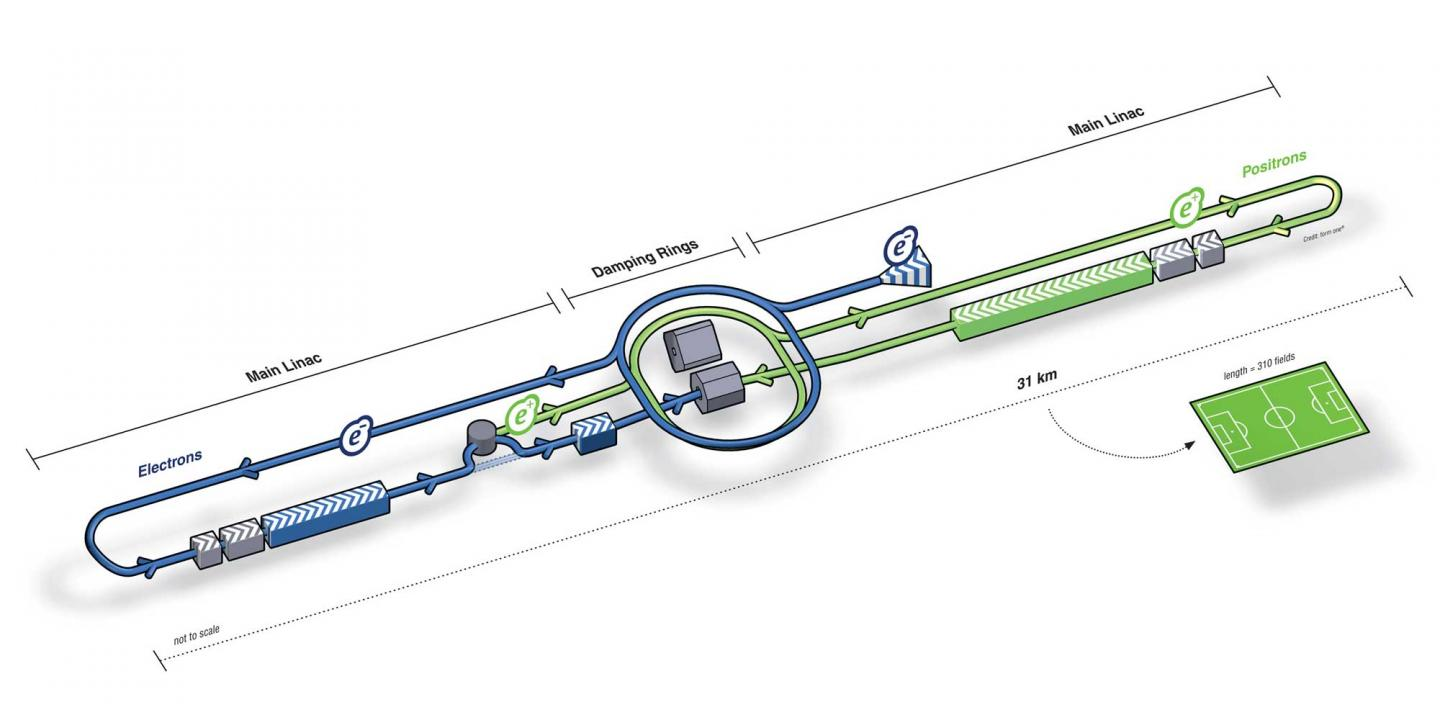
\includegraphics[width=\textwidth]{../img/ilc.jpg} 
	\caption{Schéma ILC\cite{cern:ilc}}
	\label{ilc:schema}
\end{figure}

L'objectif de l'ILC est de produire beaucoup de boson de Higgs, notamment pour découvrir s'il y en a d'autres générations du boson de Higgs. Et plus globalement pour rechercher de la nouvelle physique, par de nouveaux écarts avec le \MS.\\

À l'heure actuelle, ce projet attend les autorisations pour lancer sa construction, probablement dans les montagnes au nord du Japon. 
Et le détecteur SDHCAL correspond parfaitement aux spécifications nécessaires pour un accélérateur linéaire de ce type.
C'est pourquoi, afin de consolider sa candidature pour l'appel d'offre, l'IP2I développe aussi des programmes d'analyse de ce détecteur.

\section{Programme : \original}

% Contexte
Au début de mon stage, j'ai récupéré les codes de Guillaume \textsc{Garillot}, qui les a développé en 2021 au cours de son post-doctorat à l'IP2I. 

Son projet se divise en 3 programmes indépendants \Figure{\ref{orga:init}} :

\begin{description}
	
	\item[\texttt{miniDSTMarker}] qui permet de récupérer les données\footnote{aujourd'hui simulées mais plus tard obtenues dans le détecteur} sur le serveur distant où elles sont stockées.
	
	\item[\texttt{processor}] permet de tirer, des données brutes précédentes, des arbres \ROOT s.
	
	\item[\texttt{analysis}] utilise les méthodes des arbres binaires boostés pour effectuer une analyse statistique des arbres \ROOT issus du programme \texttt{processor}.
	
\end{description} 

% Organisation du projet initial : https://github.com/ggarillot/nnhAnalysis/tree/refactor

\begin{figure}[!ht]
	\centering
	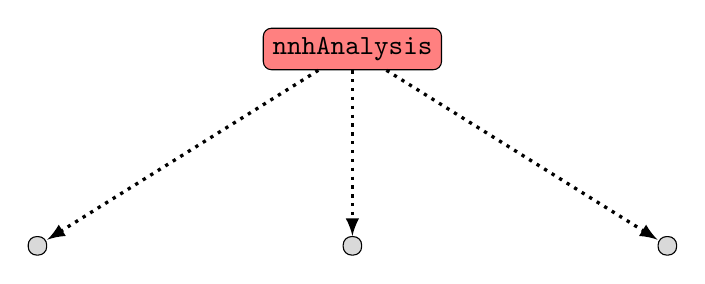
\begin{tikzpicture}

		\tikzstyle{home}=[draw, rectangle, fill=red!50, text=black, rounded corners=3pt]		
		
		\tikzstyle{directory}=[draw, rectangle, fill=gray!30, text=black, rounded corners=3pt]

		\node[home] (A) at (0,0) {\texttt{nnhAnalysis}};
		
		\node[directory] (AM) at (-4,-2.5){\minidstmarker};
		\node[directory] (AP) at (0,-2.5) {\processor};
		\node[directory] (AA) at (4,-2.5) {\analysis};
		
		
		\tikzstyle{linkDir}=[->,dotted,very thick,>=latex]
		
		\draw[linkDir] (A)--(AM);
		\draw[linkDir] (A)--(AP); 
		\draw[linkDir] (A)--(AA);
		
	\end{tikzpicture}
	\caption{
		Organisation des dossiers de mon Projet - \url{https://github.com/ggarillot/nnhAnalysis/tree/refactor}
	}
	\label{orga:init}
\end{figure}

En résumer, ce projet permet l'analyse des collisions survenues dans ce détecteur pour le projet ILC.


\subsection{Données initiales}

% données distantes : 

Malheureusement, pour le temps de ce stage, je n'ai pas obtenu l'accès au serveur, donc je n'ai pas pu utilisé \texttt{miniDSTMarker}. Je l'ai donc pas testé, ni pu développer ma propre version. C'est pourquoi, j'ai décidé de ne pas l'inclure dans mon propre code.\\

% données locales
Pour que je puisse travailler, on a mis à ma disposition certains de quelqu'un de ces fichiers, ceux des collisions à 250 \GeV. Soient 66 dossiers \Figure{\ref{data:list}} de fichiers \LCIO, où chaque nom correspond au code du type de processus \Figure{\ref{data:def}}.

\begin{figure}[h!]
	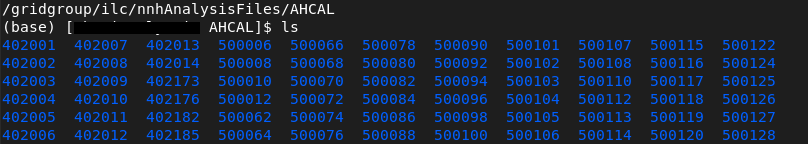
\includegraphics[width=\textwidth]{../img/listeProcessus.png} 
	\caption{Les noms des dossiers correspondent aux numéros de processus}
	\label{data:list}
\end{figure}

% Tableau des codes associés aux résultats des processus

\begin{figure}[h!]
    \centering
    \begin{tabular}{ | l | l | l | }
    		\hline
    		Type de processus & Code des processus \\
        \hline
        2 leptoniques & 500006, 500008 \\
        \hline
        2 hadroniques & 500010, 500012 \\
        \hline
        4 hadroniques & 500062, 500064, 500066, 500068, 500070, 500072 \\
        \hline
        4 semi-leptoniques & 500074, 500076, 500078, 500080, 500082, 500084, 500101, 500102, 500103, 500104, \\ 
        & 500105, 500106, 500107, 500108, 500110, 500112 \\
        \hline
        4 leptoniques & 500086, 500088, 500090, 500092, 500094, 500096, 500098, 500100, 500113, 500114, 500115, \\
        & 500116, 500117, 500118, 500119, 500120, 500122, 500124, 500125, 500126,500127, 500128  \\
        	\hline
        signal & 402007, \color{red}{402173}, \color{blue}{402176}\\
        \hline
        autres higgs & 402001, 402002, 402003, 402004, 402005, 402006, 402008, 402009, 402010, 402011, 402012, \\ 
        & 402013, 402014, 402182, 402185, \color{blue}{402173}, \color{red}{402176}\\
        \hline
    \end{tabular}
    \caption{Signification des codes des processus, \color{red}{si le signal recherché est de type \bb}, \color{blue}{si le signal est \WW}}
    \label{data:code}
\end{figure}

%if (isBB) 
%        CHANNELS_SIGNAL.insert(402173);
%        CHANNELS_OTHERHIGGS.insert(402176);
%else 
%        CHANNELS_SIGNAL.insert(402176);
%        CHANNELS_OTHERHIGGS.insert(402173);

\subsection{Conversion des fichiers initiaux en fichiers \ROOT}

Grâce au programme \processor on va pouvoir convertir les fichiers initiaux \SLCIO en fichiers \ROOT standards, afin de pouvoir les analyser.\\

On obtient ainsi pour chaque dossier de fichier de données \SLCIO un fichier \ROOT en sortie, \cad que l'on obtiendra un arbre \ROOT par type de processus.\\

Ce programme doit être robuste et donc à partir des mêmes fichiers d'entrées toujours générer des fichiers \ROOT strictement identiques.

\subsection{Analyses des collisions}

\subsubsection{Étape 1}

Avant de commencer l'analyse des fichiers \ROOT générés précédemment, on va terminer ce que le programme \processor avait commencé, et fusionner l'intégralité de ces fichiers en un seul gros fichier \texttt{DATA.root}, grâce à la commande \texttt{hadd}. 
Cette commande a été développé par le CERN et elle fusionne tous les histogrammes de différents fichiers en un seul\cite{root:hadd}. 

Donc là encore, la répétition de ce programme doit toujours générer des fichiers \texttt{DATA.root} strictement identique.

\subsubsection{Étape 2}

Pour la deuxième étape de ce programme \analysis, on va trier nos données en 4 fichiers distincts. 
Mais au lieu de les séparer par leur numéro de processus, qui est un critère numérique donc éloigné de la réalité des résultats d'une véritable expérience, on va les diviser suivant la polarisation initiale des particules incidentes, \cad l'électron et le positron à -0,8 et 0,3 ou les 2 nulles. 
Et par le type de particules produites par un boson de Higgs, \cad les canaux \bb et \WW, puisque ce sont les plus probables\footnote{Rien n'empêchera d'ajouter d'autres canaux même si le code manque encore de un peu de modularité.}.

\begin{figure}[h!]
	\centering
	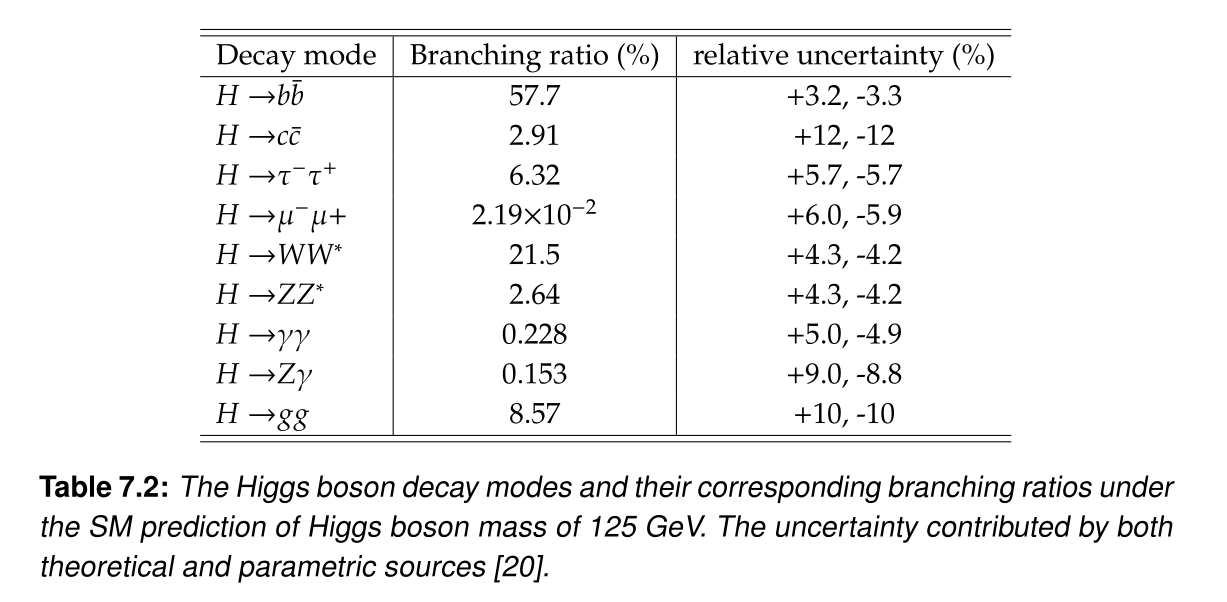
\includegraphics[width=\textwidth]{../img/Higgs_decay_125GeV.png} 
	\caption{
		Les modes de désintégrations du boson de Higgs à 125 \GeV 
		\cite{liu:tel-03405418}
	}
\end{figure}

Donc on obtient ces 4 fichiers suivants :

% Fichiers "split"

%\begin{figure}[h!]
%	\centering
%	\begin{lstlisting}
%			split_bb_e-0.8_p+0.3.root
%			split_bb_e+0_p+0.root
%			split_ww_e-0.8_p+0.3.root
%			split_ww_e+0_p+0.root
%	\end{lstlisting}
%	\label{files:split}
%	\caption{Fichiers où les évènements sont séparés en fonction des caractéristiques des polarisations des particules incidentes et des types de particules résultantes.}
%\end{figure}

\begin{figure}[h!]
	\centering
	\begin{tabular}{ | c | c | c | c | }
		\hline
		Polarisation & \multicolumn{2}{c|}{Canal} \\
		\hline
		$(e,p)$ & \bb &  \WW \\
		\hline
		$(0,0)$ & \verb|split_bb_e+0_p+0.root| & \verb|split_ww_e+0_p+0.root| \\
		\hline \cline{2-3}
		$(-0.8, +0.3)$ & \verb|split_bb_e-0.8_p+0.3.root| & \verb|split_ww_e-0.8_p+0.3.root| \\
		\hline
	\end{tabular}
	\label{files:split}
	\caption{Tous les évènements sont séparés en 4 fichiers suivant la polarisation des particules incidentes et des types des particules produites par le boson de Higgs.}
\end{figure}

Dans chacun de ces fichiers les arbres \ROOT, \texttt{TTree}, auront les variables suivantes :

\begin{description}

	\item[\texttt{isSignal} :] booléen qui indique si on considère l'évènement comme du signal ou du bruit de fond.
	
	\item[\texttt{channelType} :] entier qui représente le type de canaux de l'évènement \Figure{\ref{data:code}}:
	\begin{itemize}
		\item 2 fermions leptoniques ou hadroniques
		\item 4 fermions leptoniques ou semi-leptoniques ou hadroniques 
		\item une autre type de résultat avec un boson de Higgs
	\end{itemize}
	
	\item[\texttt{isTrain}] booléen qui confirme si l'évènement a été entrainé ou testé par la BDT.
	
	\item[\texttt{preSelected}] booléen, si l'évènement a été pré-sélectionné par la BDT.
	
	\item[\texttt{weight}] flottant qui est le poids de l'évènement en $fb^{-1}$ de la luminosité intégrée.
	
\end{description}


Pour trier les données du fichier \texttt{DATA.root}, on va utiliser des BDT pour \textit{Boosted Decision Tree}, en français, des arbres de décision boostés. 

Les arbres sont des structures de données courantes en informatique, ils sont utilisées notamment pour trier les données car ils ont une rapidité optimale en temps. 
Ici on utilise les arbres pour déterminer la nature des particules en répondant à des questions booléennes (Similaire à l'exemple \Figure{\ref{ExampleBDT}}. Et comme il n'y a que 2 issus à chaque nœud, on parle d'arbre binaire. 

\begin{figure}[h!]
	\center
	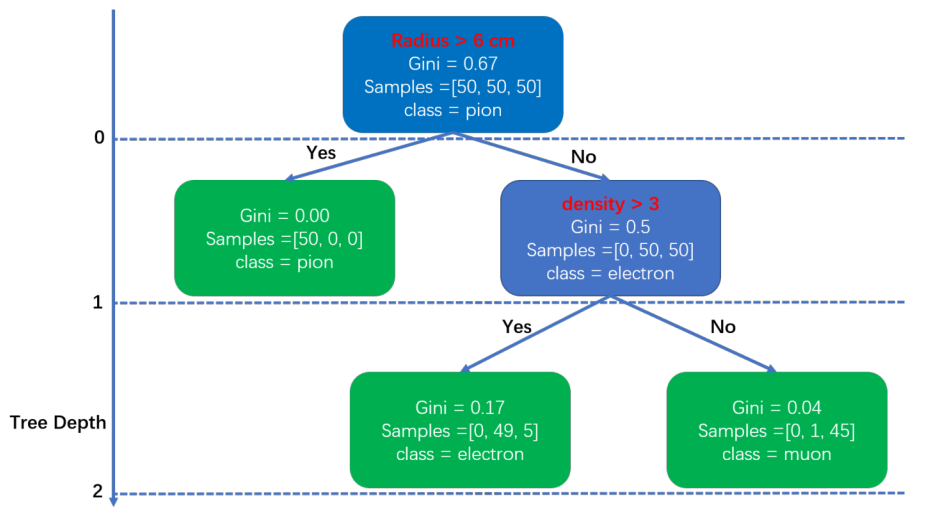
\includegraphics[width=\textwidth]{../img/ExampleBDT.png}
	\caption{Exemple de BDT \cite{liu:tel-03405418}. Ici, elle permet de déterminer de le type d'une particule}
	\label{ExampleBDT}
\end{figure}

Une fois encore, des méthodes ont déjà été développé dans l'API du CERN\cite{root:treeFriend}. Ces méthodes utilisent des paramètres générées aléatoirement afin d'augmenter la rapidité des calculs. C'est pourquoi on parle d'arbre boosté.

Mais cette fois-ci les fichiers créés sont équivalents mais pas identique. Car les BDT utilisent la génération de nombre aléatoire, ce qui engendre des variations dans les entraînements.

\subsubsection{Étape 3}

Et pour terminer, on peut enfin effectuer l'analyse à proprement parlé de nos données à partir des fichiers \texttt{split\_XX.root} précédents \Figure{\ref{files:split}}.

Cette étude se fait sur les fichiers avec une polarisation non nulle pour les particules incidentes. Car \doToList{????}


% Fichiers "model"

%\begin{figure}[h!]
%	\centering
%	\begin{lstlisting}
%			model_bb_e-0.8_p+0.3.joblib
%			model_ww_e-0.8_p+0.3.joblib
%	\end{lstlisting}
%	\caption{Fichiers du model de la BDT}
%	\label{files:model}
%\end{figure}

\begin{figure}[h!]
	\centering
	\begin{tabular}{ | c | c | c | c | }
		\hline
		Polarisation & \multicolumn{2}{c|}{Canal} \\
		\hline
		$(e,p)$ & \bb &  \WW \\
		\hline \cline{2-3}
		$(-0.8, +0.3)$ & \verb|model_bb_e-0.8_p+0.3.joblib| & \verb|model_ww_e-0.8_p+0.3.joblib| \\
		\hline
	\end{tabular}
	\label{files:model}
	\caption{Fichiers du model de la BDT.}
\end{figure}
	
% Fichiers "scores"

%\begin{figure}[h!]
%	\centering
%	\begin{lstlisting}
%			scores_bb_e-0.8_p+0.3.root
%			scores_ww_e-0.8_p+0.3.root
%	\end{lstlisting}
%	\caption{Les fichiers scores ont la réponse de la BDT : 2 variables pour chaque évènement, un booléen pour savoir s'il est sélectionné et la valeur retournée par la BDT}
%	\label{files:scores}
%\end{figure}

\begin{figure}[h!]
	\centering
	\begin{tabular}{ | c | c | c | c | }
		\hline
		Polarisation & \multicolumn{2}{c|}{Canal} \\
		\hline
		$(e,p)$ & \bb &  \WW \\
		\hline \cline{2-3}
		$(0,0)$ & \verb|scores_bb_e-0.8_p+0.3.root| & \verb|scores_ww_e-0.8_p+0.3.root| \\
		\hline
	\end{tabular}
	\label{files:scores}
	\caption{Les fichiers scores ont la réponse de la BDT : 2 variables pour chaque évènement, un booléen pour savoir s'il est sélectionné et la valeur retournée par la BDT.}
\end{figure}

% Fichiers "bestSelection"

%\begin{figure}[h!]
%	\centering
%	\begin{lstlisting}
%			bestSelection_bb_e-0.8_p+0.3.root
%			bestSelection_ww_e-0.8_p+0.3.root
%	\end{lstlisting}
%	\caption{
		%Ce fichier \ROOT contient tous les arbres \texttt{TTree} 
		%sélectionnés par la BDT comme un évènement \nnh donne 
		%$b \bbar$ ou $W \Wstar$
%	}
%	\label{files:bestSelection}
%\end{figure}

\begin{figure}[h!]
	\centering
	\begin{tabular}{ | c | c | c | c | }
		\hline
		Polarisation & \multicolumn{2}{c|}{Canal} \\
		\hline
		$(e,p)$ & \bb &  \WW \\
		\hline
		\hline \cline{2-3}
		$(-0.8, +0.3)$ & \verb|bestSelection_bb_e-0.8_p+0.3.root| & \verb|bestSelection_ww_e-0.8_p+0.3.root| \\
		\hline
	\end{tabular}
	\label{files:bestSelection}
	\caption{Ce fichier \ROOT contient tous les arbres \texttt{TTree} 
		sélectionnés par la BDT comme un évènement de \texttt{nnh}}
\end{figure}

% Fichiers "stats"

%\begin{figure}[h!]
%	\centering
%	\begin{lstlisting}
%			stats_bb_e-0.8_p+0.3.joblib
%			stats_ww_e-0.8_p+0.3.joblib
%	\end{lstlisting}
%	\caption{Statistiques.}
%	\label{files:stats}
%\end{figure}

\begin{figure}[h!]
	\centering
	\begin{tabular}{ | c | c | c | c | }
		\hline
		Polarisation & \multicolumn{2}{ c | }{Canal} \\
		\hline
		$(e,p)$ & \bb &  \WW \\
		\hline \cline{2-3}
		$(-0.8, +0.3)$ & \verb|stats_bb_e-0.8_p+0.3.joblib| & \verb|stats_ww_e-0.8_p+0.3.joblib| \\
		\hline
	\end{tabular}
	\label{files:stats}
	\caption{Fichiers des résultats statistiques pour les polarisations des particules incidentes à 0,8 pour l'électron et à 0,3 pour le positron.}
\end{figure}

Et même si cette analyse sera toujours la même \qqs les fichiers \texttt{split\_XX.root}, ces derniers étant légèrement différent d'un entraînement à l'autre les résultats statistiques \Figure{\ref{files:stats}} seront, là encore, légèrement différent mais doivent rester équivalent.

\section{Programme : \ilcsoft}

À présent, je vais vous présenter les modifications que j'ai apporté au programme \original.

Dans un premier temps, j'ai fais de la cosmétique : j'ai typé les variables, appliqué les bonnes règles de typographie et commenté les différents fichiers, classes, interfaces, fonctions, et variables globales. Ce qui m'a permis de bien comprendre les programmes et de le rendre plus lisible pour les futurs développeurs de ce code.

Ensuite je les ai modifié pour qu'il puisse s'exécuter en parallèle. En effet, \processor et \analysis mettent quelques heures à s'exécuter. Et pour tester leurs robustesses et pouvoir faire des statistiques, il est nécessaire de le faire de très nombreuses fois. Donc cette nouvelle fonctionnalité la version \ilcsoft permet un gain de temps considérable. Et plus tard, cela permettra aussi d'exécuter avec différents jeux de données (niveaux d'énergies, canaux...).

\subsection{Données}

Donc bien sûr, il s'agit des mêmes fichiers \SLCIO que pour le programme \original \Figure{\ref{data:list}}

\subsection{Programme : \processor}

Le but est toujours la conversion de chaque dossier de fichiers \SLCIO en un seul fichier \ROOT.

Pour aider à la lisibilité du programme, j'ai aussi développé une nouvelle classe qui permet de simplifier sa lecture.
Ma classe \texttt{PDGInfo} permet de manipuler plus facilement les outils du PDG, grâce à une correspondance entre les codes entiers des particules et leurs noms, ainsi que quelques méthodes et tests booléennes\footnote{\url{https://github.com/alexhxia/nnhAnalysis/blob/main/nnhProgram/ilcsoft/processor/include/PDGInfo.hh}}.

\subsection{Programme : \analysis}

La encore le fonctionnement global reste inchangé, par rapport à \original
